%-----------------------------------------------------------------------------
%
%               Template for sigplanconf LaTeX Class
%
% Name:         sigplanconf-template.tex
%
% Purpose:      A template for sigplanconf.cls, which is a LaTeX 2e class
%               file for SIGPLAN conference proceedings.
%
% Guide:        Refer to "Author's Guide to the ACM SIGPLAN Class,"
%               sigplanconf-guide.pdf
%
% Author:       Paul C. Anagnostopoulos
%               Windfall Software
%               978 371-2316
%               paul@windfall.com
%
% Created:      15 February 2005
%
%-----------------------------------------------------------------------------

% \documentclass[11pt, nocopyrightspace, numbers]{assets/sigplanconf}
\documentclass[11pt,onecolumn]{assets/IEEEtran}
% \documentclass[journal,11pt,onecolumn,draftclsnofoot]{assets/IEEEtran}

% The following \documentclass options may be useful:

% preprint      Remove this option only once the paper is in final form.
% 10pt          To set in 10-point type instead of 9-point.
% 11pt          To set in 11-point type instead of 9-point.
% numbers       To obtain numeric citation style instead of author/year.

\newcommand{\nocaptionrule}{ }
\usepackage{soul}
% \usepackage{caption} % http://ctan.org/pkg/caption

\usepackage{enumerate}% http://ctan.org/pkg/enumerate
\usepackage{caption}% http://ctan.org/pkg/caption
\usepackage{array}
\newcolumntype{L}{>{\arraybackslash}m{7cm}}

\usepackage{nimopaper}


\begin{document}

\title{\textsc{ACIDBrain}: Maintaining data consistency in microservices}

\author{
    \IEEEauthorblockN{
        Nana Pang\IEEEauthorrefmark{1},
        Wode ``Nimo'' Ni \IEEEauthorrefmark{2}, and
        Xin Chen \IEEEauthorrefmark{3}
    }

    \IEEEauthorblockA{
        Columbia University\\
        Email:
        \IEEEauthorrefmark{1}np2630@columbia.edu,
        \IEEEauthorrefmark{2}wn2155@columbia.edu,
        \IEEEauthorrefmark{3}xc2409@columbia.edu
    }
}

\maketitle


\begin{abstract}
    As software systems become more distributed and larger in scale nowadays, there is a growing need for novel architectures that are modularized, flexible, and scalable. Microservice architecture emerged as a popular software architecture where developers divide a large application into small, self-contained components (“services”). Although the separation significantly increases flexibility and reduces difficulty in development, maintaining data consistency across these isolated databases can still be be challenging. Our project targets maintaining data consistency among distributed microservices. To maintain data consistency, an event driven model called \textbf{Saga}\cite{garcia1987sagas} is often used to keep track of the data sources of each transaction. In this project, we investigate two predominant event sourcing frameworks: \textit{Eventuate} and \textit{Axon}, from an \textbf{end-user’s perspective}. We experiment with both of them by building data consistency guarantees on a dummy microservice system, and analyze the effectiveness of the two frameworks both quantitatively and qualitatively.
\end{abstract}


%------------------------------------------------------------------------------
% Content

\section{Introduction}
Large software systems have been growing rapidly and becoming more distributed. As a result, the traditional monolithic software architecture, where modules of different functionalities are closely coupled and developed by the same group of developers, is now challenged by a new architectural pattern: \textbf{Microservices}. A software system that employs microservice architecture comprises of a suite of clearly defined small services, each running in its own process \cite{lewis2014microservices}. As a result, each service can be developed by completely separated teams and using distinct technology stack, thereby decoupling the modules and parallelizing development.

In a monolithic system, all modules typically share the same backend database and enjoy the ACID (Atomicity, Consistency, Isolation, Durability) properties provided by the database \cite{gray1981transaction}. Under microservice architecture, however, each module would use a separate database to ensure good isolation among service modules, and each database might be using an entirely different technology. Therefore, large transactions that involves multiple modules, which used to run in the same database, now span across multiple databases with drastically different implementations. In this case, maintaining data consistency becomes a more complex task. \textbf{Two-phase-commit (2PC)} protocol \cite{bernstein1987concurrency} is a popular solution, where a coordinator process ensures all databases have the requested resource available before commiting the transaction. While 2PC ensures the correctness of distributed transactions, it requires all resources to be exclusively locked until the transaction finishes.

Unfortunately, in real world applications, many distributed transactions are long-lived, meaning they take much longer (in terms of hours and/or network gaps) to finish. For example, an e-commerce application may have ordering, billing, and shipping modules, and a complete transaction of purchasing an item would involve all components and would not complete until the item is shipped. In the case of these long-lived transactions, 2PC does not scale well because it locks all databases involved in the transaction and there can be many other transactions occurring in the system simultaneously.

Among the existing solutions to maintain data consistency in distributed databases of microservice systems, we chose to look at the \textbf{Saga pattern} \cite{garcia1987sagas}. There are a few arguments for Sagas over traditional consensus protocols such as 2PC. Firstly, the Saga pattern does not require synchronization of all databases in a transaction, making it more suitable for long-lived transactions. Also, Saga tends to be easier to implement than 2PC, whose logic is relatively complex.


\section{Background}
A saga is a sequence of local transactions. Each local transaction updates the database and publishes an event to trigger the next local transaction in the saga \cite{richardson2014saga}. Using this pattern, a large distributed transaction is broken into multiple local transactions that update their local databases and publish events globally to notify others, which are then coordinated by a saga. To maintain data consistency, each local transaction theoretically must be accompanied by compensatory transaction. As a result, the saga can rollback the large transaction by executing these compensations in a reverse order.

In general, there are two types of sagas: \textit{choreography-based} and \textit{orchestration-based}. An orchestration-based saga is a standalone object that coordinates multiple service in a centralized manner, whereas choreography-based saga is implemented by each local transaction publishing domain events that trigger local transactions in other services \cite{richardson2014saga}.

The use of microservices and sagas also motivates the overall architectural pattern to deviate from the traditional layered architecture. \textbf{Event sourcing} and \textbf{Command Query Responsibility Segregation (CQRS)} are often used to fully implement sagas. Since sagas coordinate local transactions by publishing events after updating local datastores, it is vital for the publication and update to be atomic - otherwise the system ends up in an inconsistent state. Event sourcing is used to enforce atomicity of events publishing and datastore updates. Event sourcing persists the state of entity as a sequence of state changing events. Whenever an entity changes, a new event is appended. The final state of each entity must be consistent since adding a single event is atomic. Therefore, we don’t need compensation rollback to maintain data consistency but persist events in an event store, adding or retrieving event when an entity is changed.

Unfortunately, with multiple local databases involved in one event store, querying these databases becomes much more difficult to implement than in a monolithic system. Since the current state of all entities are stored as a sequence of changing events rather than a static record, it is difficult to obtain the most up-to-date state of a certain entity. To mitigate the complexity, the CQRS architecture is often used in implementations of sagas. CQRS separates queries from commands/modifications to the datastore


\section{Existing Implementation of Sagas}
During our early research on Microservices, we found a number of online documents about Microservices, but most of them only explain the architecture style of Microservices which more accessible but remain too high-level to guide implementation. For example, searching “Microservices” on Google gives around 1,700,000 results, “Microservices example” only gives about 706,000 results. Furthermore, “Microservices data consistency” gives only 62,300 results. Our project aims to find out more about what technology can be used in implementing Microservices with data consistency guarantees, which is a relatively less discussed topic with fewer alternatives in terms of concrete implementations.

\hl{\textbf{Which systems we have chosen and why: }} Having decided to investigate Sagas, we looked into the existing implementations of Saga pattern for microservices. Among them, we picked \textbf{Eventuate} and \textbf{Axon}, which are the most popular and well maintained. We summerize the two frameworks briefly here:

\begin{itemize}
    \item \textbf{Axon framework} \cite{axon} is a Java based framework for building scalable and highly performant applications. The main notion is the event processing which includes the separated Command bus for updates and the Event bus for queries. According to an original Axon author’s response on StackOverflow \cite{comparison}, Axon has been around for about 8 years and is being used by many systems in production since then. Axon has extensive support for Spring. Yet Spring is not required for Axon, it made configuration easy with Spring annotations.
    \item \textbf{Eventuate} \cite{eventuate} is a platform that provides an event-driven programming model that focus on solving distributed data management in microservices architectures. The framework stores events in the MySQL database and it distributes them through the Apache Kafka platform. Eventuate is a framework that has integration with Gradle and Maven project. Therefore, we have implemented our prototype using Spring and Maven.
\end{itemize}

There are already comparisons online of the two frameworks \cite{comparison, stefanko}. All of we could gathered, however, were written by implementers of transaction frameworks. For example, \cite{stefanko} was written by the a member of the Narayana team within Red Hat, which also has a similar implementation. Therefore, in this project, we would like to evaluate the end-user experience of using Saga frameworks to implement data consistency in microservice systems.

\hl{\textbf{How we obtained the systems:}} Since both Eventuate and Axon frameworks themselves are freely available on the internet (it seems that some of other related services are not, we obtained them through their official websites \cite{axon, eventuate}.


\section{Method}
\begin{figure}[H]
    \centering
    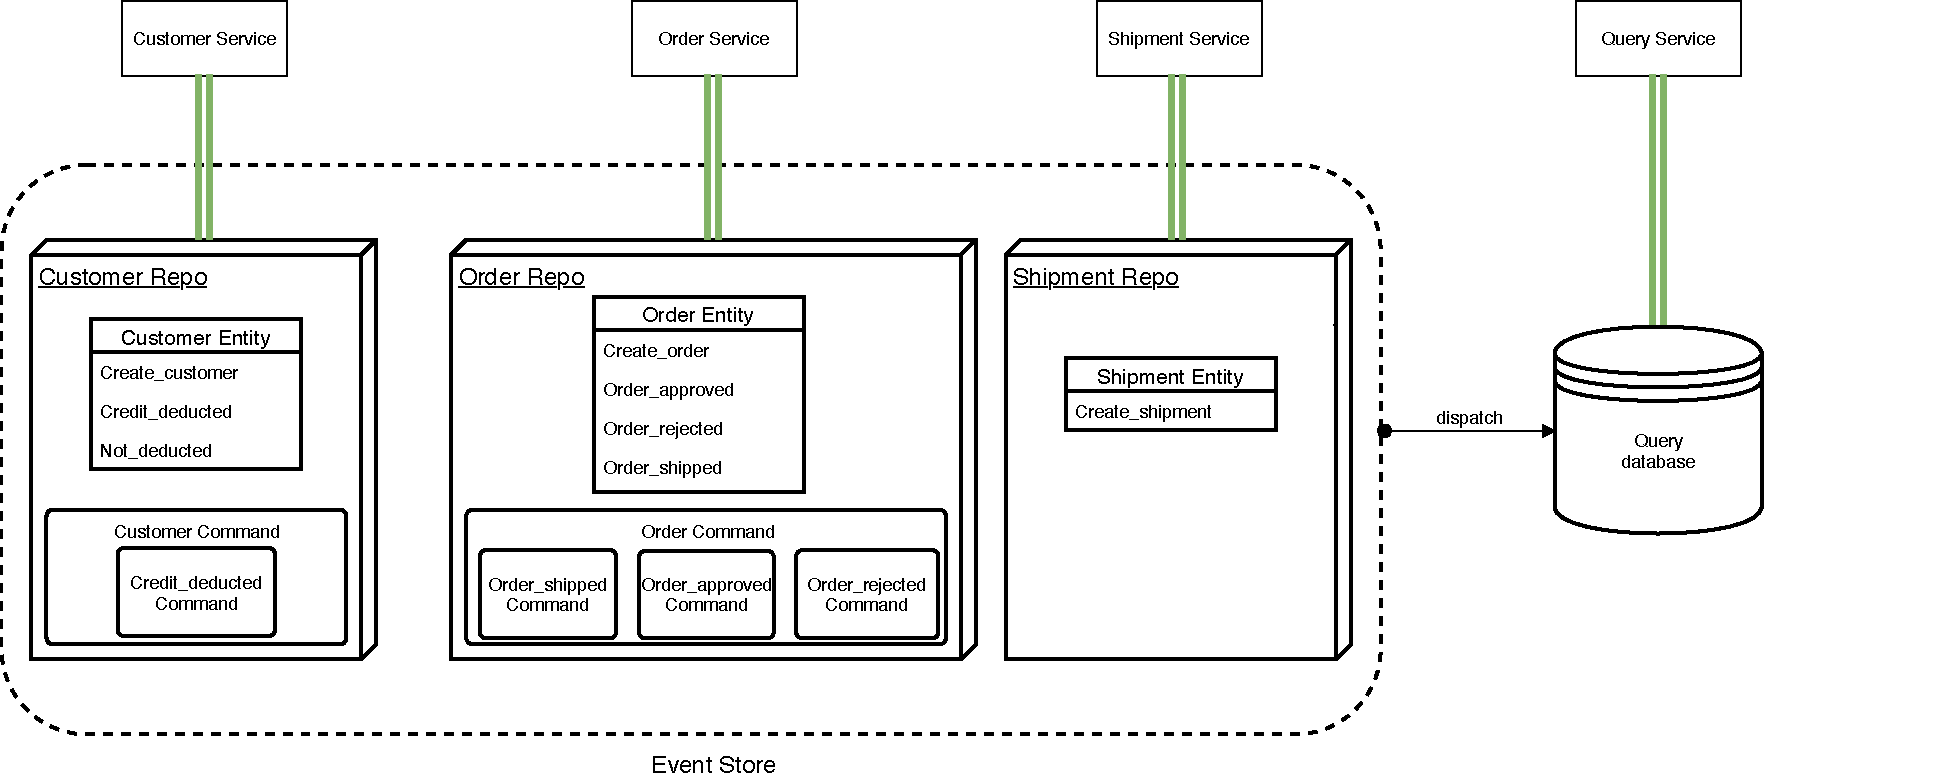
\includegraphics[width=17cm]{assets/arch.pdf}
    \nocaptionrule \caption{\label{fig:arch} Overall structure of the e-commerce prototype}
\end{figure}

To evaluate the usability of Axon and Eventuate frameworks, we take on both quantitative and qualitative approaches. We implemented a dummy e-commerce system with a business logic that requires multi-database transaction in a rational manner and is very common in the real world. The general workflow of the system is the following:

% {\fontfamily{pcr}\selectfont
\begin{enumerate}
    \item Create a customer with name and credit limit
    \item Create order
    \begin{itemize}
        \item If order amount does not exceed customer credit limit, approve order and subtract credit.
        \item If order amount exceeds customer credit limit, reject order and maintain credit unchanged
    \end{itemize}
    \item If order is approved, create shipment, order status change as shipped.
\end{enumerate}
% }

The system starts off with no data consistency guarantees. As the experiment, we implement data consistency using the two frameworks separately by two team members (Nana and Xin). To evaluate the usability quantitatively, we plan to record the following data:

\begin{itemize}
    \item Total lines of Java source code (SLOC)
    \item Size of the systems on the disk
    \item Estimated time taken to implement the improvement
    \item Total time spent on the web (also separately on GitHub, StackOverflow, documentation website and other related reference sites)
    \item Documentation: total number of words, estimated coverage of the framework APIs
    \item Performance and stability: we use Artillery to load test the two implementations using Axon and Eventuate. If significant difference detected, we can also report system resource usages (CPU usage and network respond time).
\end{itemize}

Qualitatively, we will report our experience using the two frameworks, provide some more anecdotal cases of tasks such as reading the documentation, and showcase some snippets of code to discuss their API designs.


\section{Results}
\subsection{User comments}

This section includes first-person accounts from two members of our team who implemented data consistency for the same e-commerce prototype, respectively.

\paragraph{Eventuate (Nana)}

\begin{itemize}
    \item \textit{Pros \#1}: Eventuate framework maintains high modularity by dependency injection, using tags such as \texttt{@even\-tentity}, \texttt{@event}, \texttt{@aggregate}, \texttt{@eventsubscriber} to define unit field. Each of these fields has a generic abstract class to inherit, which makes user easier to organize system structure. Decoupling is one of the benefits in modularity. Due to the high modularity in Eventuate, it also has low coupling as well.
    \item \textit{Pros \#2}: Eventuate persists transaction atomicity by using sequence of state-changing events in entity. Whenever the state of a business entity changes, a new event is appended to the list of events. Eventuate workflow includes command processing and event publishing while updating entity status. This design reconstructs an entity’s current state by replaying the events. Since saving an event is a single operation, it is inherently atomic.
    \item \textit{Pros \#3}: Eventuate provides clean and concise samples for users to start up their application. Those samples have great code legacy in modularity, which divides a large system into different layers and helps user to find useful information efficiently.
    \item \textit{Cons \#1}: Eventuate is difficult to configure or saying, difficult to configure without Docker. Unlike Axon, which could download the released package and run locally, Eventuate provides services through Docker and Docker Compose. Therefore, it requires user to learn how to use Docker first. Eventuate also provides free AWS platform to run their services without local configuration. But it takes them 2 weeks to respond my request for AWS access key, which is quite slow.
    \item \textit{Cons \#2}: One key drawback of Eventuate is that it uses too many extra products such as Zookeeper and Kafka to implement functionality. In our system, we have implemented 4 services but using Eventuate requires 5 extra services to run first. The resource consumption such as CPU utilization is higher than Axon. Also, during our experiment, we found that some services in Eventuate is not stable and often stop running in Docker automatically. It is possible that Eventuate has bug not found, which makes it unstable or not compatible with Docker.
    \item \textit{Cons \#3}: Even though the sample code is well organized in Eventuate, its tutorial is worse than Axon or any other framework tutorial I have read before. The documentation merely defines the syntax of the API, but \textbf{not} the underlying semantics – the intents of the functions and their effects on the whole system. Also, the tutorial covers only a small section of implementation in Eventuate. For example, EventUtil is frequently used in sample code but never explained in tutorial.
\end{itemize}

\paragraph{Axon (Xin)}

\begin{itemize}
    \item \textit{Pros \#1}: Building with Axon is highly modular, each entity or a type of entities is represented by an aggregate. Inside a aggregate class, we declare its attributes and aggregate id. \texttt{Commands} and \texttt{Events} are also classes that capture what actions to take. Axon extensively provide annotation support, such as \texttt{@aggregate}, \texttt{@commandHandler}, \texttt{@eventSourcing}, which made it easy to the developers.
    \item \textit{Pros \#2}: Axon official website \cite{axon} has documentations that explain terminologies and provide code samples. It is a well-documented framework, and updates regularly.
    \item \textit{Pros \#3}: Configuration with Spring is also easy. Spring is not a prerequisite for using Axon, so developers have the flexibility to make their own decision based on personal preference.
    \item \textit{Pros \#4}: Axon is open-source and freely available, there are big organizers such as banks using Axon in their core system. This also indicates that Axon is a fairly mature framework.
    \item \textit{Cons \#1}: Hard to handle mistakes in event handlers locally: if an error appears in one of the event handlers, there is no other way than reconstructing past states. The replaying process may take a long time depending on data size.
    \item \textit{Cons \#2}: Since commands and events are immutable, they have to be defined by Kotlin (Kotlin is a statically typed programming language that runs on the JVM and also can be compiled to JavaScript source code or use the LLVM compiler infrastructure.) and put into core api. Although Kotlin allows users to concisely define each event and command on a single line, it may add extra work for people who has no experience with Kotlin.
\end{itemize}


\subsection{Code examples}

\begin{figure}[H]
    \centering
    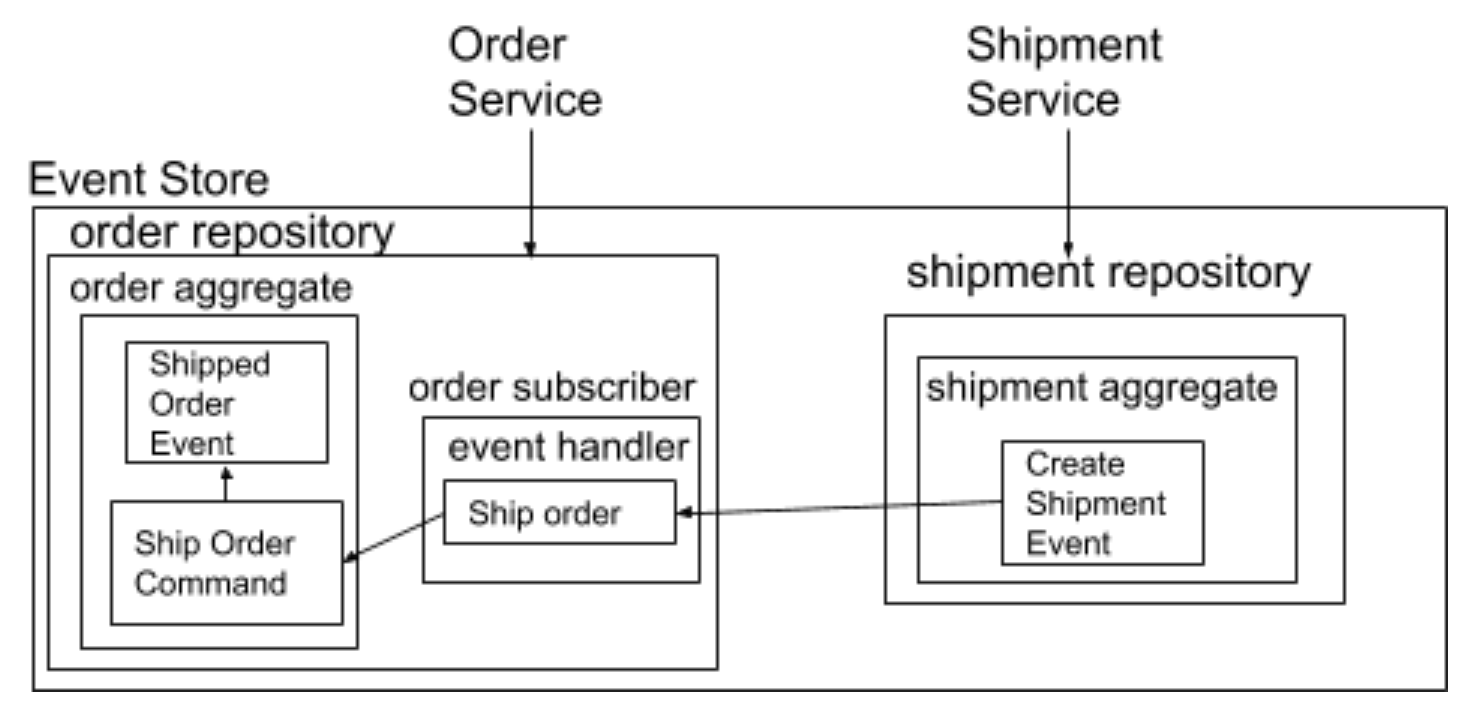
\includegraphics[width=9cm]{assets/README-d8970.png}
    \nocaptionrule \caption{\label{fig:code-example} Content in event store for shipping and ordering service}
\end{figure}

\subsubsection{Eventuate}
\begin{enumerate}[i]
    \item Create basic components of the service: \texttt{ShipOrderCommand}, \texttt{OrderShippedEvent}, and \texttt{ShipmentCreated\-Event}. (Listing \ref{code:eventuate-basic} in Appendix)
    \item Set up event handler method in order service to monitor \texttt{ShipmentCreatedEvent} and invoke \texttt{ShipOrder\-Command} if \texttt{ShipmentCreatedEvent} is generated. (Listing \ref{code:eventuate-handler})
    \lstinputlisting[language=java, caption={Event handler example in Eventuate}, label=code:eventuate-handler]{code/even-handler.java}
    \item Overload \texttt{process} function in \texttt{ShipOrderCommand} class and \texttt{apply} function in \texttt{OrderShippedEvent} class in \texttt{Order} aggregate to generate \texttt{ShipmentCreatedEvent} and change order status. (Listing \ref{code:eventuate-event})
    \lstinputlisting[language=java, caption={Overloading \texttt{apply} and \texttt{process} in Eventuate}, label=code:eventuate-event]{code/even-event.java}
\end{enumerate}

\subsubsection{Axon}

\begin{enumerate}[i]
    \item Basic unit is aggregate. An aggregate is an entity or a collection of entities. It needs to have an aggregate id.

    \lstinputlisting[language=java, caption={\texttt{Aggregate} example in Axon}, label=code:eventuate-handler]{code/axon-aggregate.java}

    \item Command classes are identified by the aggregate id it relates to.

    \lstinputlisting[language=java, caption={\texttt{Command} example in Axon}, label=code:eventuate-handler]{code/axon-command.java}

    \item Each aggregate defines their own commandHandlers, each eventSourcingHandler corresponds to one type of commandHandler. For the example below, we assign orderId to this order object only if the command is of type \texttt{FileOrderCommand}.

    \lstinputlisting[language=java, caption={Handlers defined in Axon}, label=code:eventuate-handler]{code/axon-handler.java}

    \item After the order goes through, Shipment aggregate will receive \texttt{prepareShipmentCommand}, and apply \texttt{ShipmentPreparedEvent} for this order.
    \lstinputlisting[language=java, caption={Shipment aggregate in Axon}, label=code:eventuate-handler]{code/axon-ship.java}

    \item The eventSourcingHandler for \texttt{ShipmentPreparedEvent} is called after applying the event successfully in the commandHandler.
    \lstinputlisting[language=java, caption={Shipement event handler in Axon}, label=code:eventuate-handler]{code/axon-eventsource.java}
\end{enumerate}

\subsection{Load test and Resource Consumption}

\begin{table}[H]
    \begin{center}
        \begin{tabular}{ | m{2cm} | l | l | }

            \hline
            & Axon & Eventuate \\

            \hline
            CPU Utilization &
            $66.4\%$ &
            $19.6\%$ \\

            \hline
            Median Request Latency &
            $58.4$ ms &
            $345.6$ ms \\

            \hline
            Service Breakdown & No & Yes \\

            \hline

        \end{tabular}
    \end{center}
    \caption{Comparison between Axon and Eventuate}
    \label{table:load}
\end{table}

To test for the \textbf{stability} of Axon and Eventuate, we used Artillery to load-test the prototypes. Since data consistency is guaranteed by the framework and thus is not the central concern for this particular test, we only test for a part of the whole purchase transaction: \textit{assuming an existing user, place an order with the ID of that user}. In this test, we repeatedly create new orders under the same customer and test whether the system can handle the traffic load. In the load-test for Eventuate, \textbf{12000} requests are sent within 120 seconds, and all request succeeded. However, the same load completely broke the Evantuate version of the same prototype. Note that although the requests were never successful, no partial transactions were performed by Eventuate, and the system is indeed consistent. Therefore, Evantuate was tested using fewer number of requests. The results are summarized in Table \ref{table:load}.

\subsection{Development tatistics}

The following table summarizes statistics about the two prototypes and development of them. Fully LOC information can be found in Appendix (Listings \ref{code:eventuate-loc}, \ref{code:axon-loc}).

\begin{table}[H]
    \begin{center}
        \begin{tabular}{ | m{2cm} | l | l | }

            \hline
            & Axon & Eventuate \\

            \hline
            Total Time Spent &
            $41.3$ hours &
            $63.5$ hours \\

            \hline
            LOC (Java) &
            1189 lines &
            2304 lines \\

            \hline
            LOC (Total) &
            2300 lines &
            3227 lines \\

            \hline

        \end{tabular}
    \end{center}
    \caption{Development statistics of two prototypes}
    \label{table:stats}
\end{table}

During the development, we also attempted to search on \texttt{http://stackoverflow.com/} for either Axon or Evantuate related questions, As of May 4, 2018, searching or ``Axon'' gives \textbf{336} results\footnote{https://stackoverflow.com/search?q=axon}, whereas searching for ``Eventuate'' gives \textbf{51} results\footnote{https://stackoverflow.com/search?q=eventuate}.


\section{Discussion}
\subsection{Comparing Axon and Eventuate}

\begin{table}[H]
\begin{center}
  \begin{tabular}{ | m{2cm} | L | L | }
    \hline
    & Axon & Eventuate \\

    \hline
    Aggregate &
    Use \texttt{@Aggregate} annotation in the beginning of class. Place  \texttt{@Aggregate\-Identifier} on top of unique identifier for this aggregate. Aggregate contains \texttt{@commandHandler} annotation and \texttt{@eventSourcingHandler} and overload apply method to update entity state.  &
    Extend  \texttt{ReflectiveMutableCommand\-ProcessingAggregate<aggregate, command>} class to define aggregate. Overload process and apply method in aggregate update entity state. \\

    \hline
    Event &
    No class to define events. Prototypes in core api by Kotlin &
    Use \texttt{ @EventEntity(event=event\_n\-ame) } annotation in Event class \\

    \hline
    Command &
    User defined command class which uses \texttt{@TargetAggregate\-Identifier} to connect with Aggregate &
    Extend  \texttt{Command class} to define command \\

    \hline
    Saga &
    Is a special type of Event Listener that manages a business transaction. Sagas are classes that define one or more \texttt{@SagaEventHandler} methods. All Sagas must implement the Saga interface. &
    Use \texttt{@EventSubscriber} annotation to define event listener in each service. Use \texttt{@eventhandler} method annotation to define transaction message. \\
    \hline

  \end{tabular}
\end{center}
\caption{Comparison between Axon and Eventuate}
\label{table:compare}
\end{table}

As shown in Table \ref{table:compare}, we can find some syntactic difference between Axon and Eventuate. Axon requires users to define their own command using \texttt{@TargetAggregateIdentifier} annotation corresponding to \texttt{Aggregate} identifier. Therefore, command and aggregate are combined using annotation in Axon. Eventuate has much clearer structural architecture. For instance, event, entity and command are units defined as generic abstract class in Eventuate. User could implement them without knowing \texttt{Aggregate} definition. Therefore, command is coupling with \texttt{Aggregate} in Axon, while decoupling in Eventuate. So, Axon has more complicated syntax and lower decoupling ability.
Also, since Axon and Eventuate are primarily CQRS based frameworks, they require some additional handling for the saga execution. In Axon, saga is still the aggregate which means that it consumes commands and produces events. This may be an unwanted overhead when the application does not follow the CQRS domain pattern. The same applies to Eventuate but as the communication is shadowed through the messaging channels it does not force the programmer to follow CQRS. Instead, event handler methods in command service and query service are defined separately in Eventuate, which provides more flexibility of system architecture. So, we can say that Axon is more fixed while Eventuate is more flexible.

\subsection{Prospective User Community}
\hl{\textbf{Target user community and value added}}

The user community of Microservices is large and keeps growing. As we presented, Microservices has lots of advantages. Even though Microservices architecture shares ideas with other models such as Service-Oriented Architecture, it has attracted much attention from big companies such as Amazon, Uber, and Netflix. Thus, for software developers, learning and implementing Microservices architecture could be a increasingly popular requirement in the future.

To apply Microservices in real-world products, we need to deal with tradeoffs of such a decentralized system. Importantly, data consistency across distributed databases is vital for many business systems. In certain systems, it is conceptually and realistically difficult to perfectly divide your software into completely independent and isolated services. As a result, data transactions that span two or more services are inevitable in such cases. As the amount of Microservices architecture increases, the importance of maintaining data consistency in Microservices will be increasing as well.

\hl{\textbf{What do your results show that was not already known}}

\hl{\textbf{How members of the user community will find out about your study}}

\hl{\textbf{Accessing our results}}

Since the concept of microservice is relatively young (the term was first used in 2011 \cite{wiki:micro}, the topic of maintaining data consistency is under-researched in the academia and implemented mostly in an ad-hoc fashion. Our study investigated two of the few existing software frameworks that aim to achieve data consistency and work well with systems of microservice architecture. More importantly, instead of evaluating from an implementer’s point of view such as \cite{comparison, stefanko}, we experiment with these frameworks as end-users and attempt to evaluate the usability of them both quantitatively and qualitatively. Therefore, we believe that the results from this study can be shared to the user community of Axon, Eventuate, or any frameworks alike, and provide a reference point for choosing one of them. Our GitHub repo\footnote{https://github.com/nanahpang/Microservices \hl{project deliverable}} contains original documents and prototypes that we built, and it is freely accessible to everyone.

\subsection{\textsc{ACIDBrain} Team Comments}

\subsubsection{Nana}
\begin{itemize}
    \item \textbf{Responsibilities}:Implement original prototypes using Java and Spring. Implement prototype with customer, order, shipment and query services by using Eventuate framework. Test Api through Swagger UI and deploy application on AWS.
    \item \textbf{Comments}: At the beginning of development, I found  some methodology such as Saga pattern, CQRS view and event sourcing are difficult to define or distinguish. Online resource of these concept is incomplete and vague. During the implementation process, I stuck at the configuration and building part for a long time, since I am not familiar with Spring cloud and Docker which is used by Eventuate. Therefore, I chose to study from an existed sample Eventuate provided, analyzing its code structure and labeling functionality within each modules. Since I have experienced Java and Spring development before, I started to make some progress. After implement the shipment service, I realize that Eventuate doesn’t need compensation function as I assumed because it maintains entity status by logical checking and only apply the eventually consistent event in event store. All the event states are remained unchanged after initialization and compensation is handled by adding new event such as order-approve-event and order-reject-event after order-created-event.This feature has both pros and cons. It simplifies the complexity of understanding system workflow but adds extra nodes in code implementation. But it is always difficult to find a perfect solution. Every method has its pros and cons. Therefore, in project report, I have discussed pros and cons of Eventuate and compared usability of Eventuate and Axon. This topic is related to my midterm paper. I didn’t realize the data consistency issue in Microservices architecture until presentation. It is my pleasure to learn more about Microservices and implement a system in Microservices. I hope our project could be helpful to other end-users who are interested in software architecture as well.
\end{itemize}

\subsubsection{Nimo}
\begin{itemize}
    \item \textbf{Responsibilities}: Maintaining AWS server and docker, load-test scripting, (part of) implementation of original prototype, development statistics gathering, report drafting, and presentations.
    \item \textbf{Comments}: My software engineering experience has primarily been in academic settings. Therefore, reading about and experimenting with newer technologies from the industry was eye-opening to me. Interestingly, patterns such as microservices become popular because of not just its technical benefits, but also faster deployment and more distributed development model, both being more business and human related concerns. One of the first problem that we encountered was the lack of strict definitions of many terms such as event sourcing, sagas, or microservices, which is expected given that these terms are not used rigorously. Later on, we experienced roadblocks when setting up the development environment using AWS, docker, Maven, and other tools. The technical overhead significantly impaired the complexity of our prototype system and the later improvement on them using the two frameworks. Since both Axon and Eventuate are designed to solve issues in large, complex systems, it might be more reasonable to experiment them  on a larger system with more services and significantly more complex and coupled business logic, which we unfortunately did not have. Finally, some comments on usability of frameworks: Frameworks exists to ease software development, among many other reasons. As we demonstrated in the project, there are still highly visible flaws in the design of the APIs of both Eventuate and Axon. There is always a human-factor in the design of frameworks. As API usability \cite{daughtry2009api} gets more attention in the field of software engineering and Human-Computer Interaction, more principles and guidelines should be developed for better design of them.

\end{itemize}

\subsubsection{Xin}

\begin{itemize}
    \item \textbf{Responsibilities}: Learning and implementing original prototypes using Axon framework. Modify original prototypes to adapt axon environment. Test order, invoice, shipment services by posting and getting requests on Swagger. Axon development time statistics tracking and documenting obstacles.
    \item \textbf{Comments}: I have little preliminary experience in Spring, so I spend fairly large amount of time in learning Spring structure. There were a lot of axon-specified annotations to add in my code. Although axon is a more mature framework than eventuate, there is little small-scale complete code samples. Building with axon requires a throughout understanding of CQRS architecture, and this is where I harvested the most from this project. With reading other axon project codes, along with axon official guideline, I finally got the rationale of axon logics and got the code running. I can say that axon is not a very user friendly framework as users need to implement axon interfaces. However, a developer with system level development experience may have a different perspective. Before this course, I always heard things about microservices but never had a change to work on a project. Knowing the technique of how to keep data consistency between microservices, I can transfer this skill set further into distributed systems.
\end{itemize}


\section{Conclusion}
In this project, we experimented with and evaluated two existing frameworks, Axon and Eventuate, that implements data consistency for distributed transactions using Saga pattern. The two frameworks are similar in principle. Both of them implement Saga pattern and CQRS view. From a end-user’s point of view, however, there are identifiable tradeoffs in choosing either of the frameworks. In short, Eventuate, being the newer design of the two, is more user-friendly and provides better decoupling of components in the system. However, comparing to Axon, it is more unstable and performs worse due to its shorter development time. Axon, on the other hand, has a less-friendly API with tighter coupling of components such as handlers for commands and events. Moreover, between the two frameworks, Axon is relatively more light-weight because it only provides a skeleton structure, whereas Eventuate provides functional implementation for most parts of the system and therefore contains more scaffolding code.




%------------------------------------------------------------------------------
% bibliography

\FloatBarrier{}
% prevent figures breaking the reference section

\bibliographystyle{unsrt}
\bibliography{bibliography}

%------------------------------------------------------------------------------
% appendix

\appendix

\subsection{Code snippets of Eventuate prototype}

\lstinputlisting[language=java, caption={Basic building blocks in Eventuate}, label=code:eventuate-basic]{code/even-basic.java}

\subsection{LOCs of two prototypes}

\lstinputlisting[caption={LOC statistics of the prototype built using Eventuate}, label=code:eventuate-loc]{code/loc-eventuate.txt}

\lstinputlisting[caption={LOC statistics of the prototype built using Axon}, label=code:axon-loc]{code/loc-axon.txt}


\end{document}
